\documentclass[11pt]{article}
\title {Quantifying the overlap of sharks, enforcement and illegal fishing inside one of the world’s largest marine protected areas}
\author{Emma Deeks}
\date{10 Dec 2019}
\usepackage[margin=2cm]{geometry}
\usepackage{graphicx}
\usepackage[]{lineno}
\usepackage[backend=biber,style=authoryear,bibencoding=utf8]{biblatex}
\setlength{\parindent}{0em}

% bibliography secion %

\addbibresource{miniproject.bib}

\begin{document}
	
	\begin{titlepage}
		
		
		\centering % this centers everything on the page
		
		%\vspace  % Whitespace at the top of the page 
		
		
		% --------------------------
		%% TITLE
		
		\vspace*{5\baselineskip}
		
		\rule{\textwidth}{1.6pt}\vspace*{-\baselineskip}\vspace*{2pt} % Thick horizontal rule
		\rule{\textwidth}{0.4pt} % Thin horizontal rule
		
		\vspace{0.75\baselineskip} % Whitespace above the title
		
		{\LARGE QUANTIFYING THE OVERLAP OF SHARKS, \\ ENFORCEMENT AND ILLEGAL FISHING \\
			INSIDE ONE OF THE WORLDS LARGEST \\ MARINE PROTECTED AREAS \\} 
		
		\vspace{0.75\baselineskip} % Whitespace below the title
		
		\rule{\textwidth}{0.4pt}\vspace*{-\baselineskip}\vspace{3.2pt} 
		\rule{\textwidth}{1.6pt} 
		
		\vspace{2\baselineskip} 
		
		% ---------------------------------
		%% SUPERVISORS & CONTACT EMAIL
		
		Supervisors: \\
		Dr. David Jacoby, Zoological Society of London \\ 
		Dr. James Rosindell, Imperial College London 
		
		
		
		\vspace{1.5 \baselineskip} % Whitespace between text
		
		Contact: \\
		ead19@imperial.ac.uk
		
		\section{Key Words}
		\begin{itemize}
			
			\item Pelagic predators
			\item Conservation
			\item Illegal fishing
			\item Spatio-temporal trends
			\item Modelling 
			\item Marine Protected Areas
		\end{itemize}
		
	\end{titlepage}
	
	\linenumbers
	
	\section{Introduction}
	\noindent

	
Functional responses describe the way in which a predator responds to changing densities of prey \cite{Holling1959}. This is important as it is a key regulating factor for population dynamics. The rate at which a predator kills its prey at different densities ultimately determines the efficiency of a predator in regulating population densities of prey. \cite{Murdoch1975}. \cite{Holling1959} described three types of functional responses curves, the first, an increasing linear relationship indicating a constant rate of predation. The second is a decerlating curve which indicates saturation at a certain level, e.g. saturation of predator eating prey, and the third is a sigmoidal relationship which indicates a increased rate of prey killing, or, positive density dependant prey mortality. \cite{Pervez2005}. It has been observed that often, the type II functional responsed is favoured in predator prey relationships, that is a curve which starts at low prey densities and as the prey density increases so does the predation rate linearly until it saturates at an upper limit \cite{Jeschke2002}. Functional response models are used, often above linear models, as they incorporate two parameters which are handling time (time required to attack, consume and digest prey) and attack/search efficiency of a predator to a prey \cite{Fathipour2016}. Functional response models can be applied in ecology when predicting future population densities of predators and prey within the functional response relationship as well as what happens to each member of the relationship when densities of one changes \cite{Jeschke2002}

Functional responses can be modelled in a phenomenological way, such as the Holling type II model \cite{Holling1959}, which cannot explain the underlying mechanism of the curve they produce, the parameters cannot be mechanistically explained, but still produce the traditional type II response curve. The second model is the mecanistic model where the parameters involved can all be mechanistically explained \cite{Jeschke2002}.

Whilst these models do well to try and fit functional responses between species, many other factors can potentially effect the functional responses between species in space and time. Whilst the shape of the functional response curve is dependent on several charactistics such as the encounter rare, capture efficiency and the handling time of the predator \cite{Holling1965}, these various characteristics are often species dependant as species vary in a number of attributes such as size and space \cite{Elliott2003}. To account for these varying chracteristics studies such as \cite{Aljetlawi2004}  have undertaken studies to include characteristics of species such as size into functional responses to produce a size dependant functional response. Other studies such as \cite{Pawar2012} highlighted the importance of considering the dimensions in which consumers encounter resources, for instance, 2D dimensions involve terrestrial habitats whereas 3D dimensions include arial and pelagic encounters. From studies such as these it highlights the importance of not only choosing the best model to accurately describe functional response, but also emphasises the importance of considering species on a more individual basis, for instance, the habitat they occupy and the dimension in which predators encounter resources. 

This study looks at two mechanistic and two phenomological models and fits them to a functional response dataset from \cite{Pawar2012} study in order to find whether mechanistic or phenological best describes functional response data. This study also looks at the dimensions and habitat functional response curves are in and aims to test whether the model type varies based on this. 

The key questions of this project are:
	\begin{itemize}
	\item How well do different mechanistic and phenpmenological mathmathical models fit functional response data across different species
	\item How does habitat effect these model fits? 
	\item How does the dimension the predator ecounters the resource effect model fits? 
	\end{itemize}


	\section{Methodology}
\noindent

The four models fitted to the functional response data was the cubic, quadratic, Holling Type II and Generalised functional response model. 

The first script in the workflow is a python script that;
	\begin{itemize}
	\item Imports data and subsets based on relevant columns for study, removes any missing values and saves the resulting dataframe to a csv file 
	\end{itemize}

The second script in the workflow is an R script that;
\begin{itemize}
	\item Imports the modified csv file and nests the data using the 'dplyr' package 
	\item It then runs a function for obtaining initial start values on the nested data and outputs a dataframe of start values called 'datatouse'
	\item It defines the functions of the Holling Type II functional response as 'powMod' and the generalised functional response model as 'GenMod'
	\item it then runs a for loop that samples the starting values to find the optimum starting value for each functional response to use for the model fitting
	\item it then runs a for loop which outputs two tables, 'optimisedtable.csv' has the best fit model for each of the functional response curves as well as the habitat and dimension the species of each funtional response curves is in. 'MergedOptTable.csv' has every model and their associaiated AIC values for stats in the plotting script 
	\item Finally, this script plots all four models on a sample functional response model as an ilustrative on model fits. (Figure 1)
\end{itemize}

The third script in the workflow is a python script that;
\begin{itemize}
	\item Imports 'MergedOptTable.csv' and 'optimisedtable.csv' for statistical analysis and plotting of data for results 
\end{itemize}


	\section{Results}
\noindent

Out of the 215 curves fitted with the four different models 60\% of the best fits were mechanistic models, in this study, the cubic and the quadratic model. Whilst it may be expected that the phenomenological models would be a more suitable fit due  to the optimised start parameters, the handling time (h) and the            (a), as well as the spatial parameter encompassed in the generalised functional response model. Potentially, the method for optimising starting values of these models were involved in why these models were less successful then the mechanistic models. As well as this, the spatial parameter q was set to 0.75, as used in \cite{Pawar2012} paper of functional responses. Varying or optimising this spatial parameter may have potentially led to decreased model fits. As well as this, having the spatial parameter set to 0.75 means the line produced closely resembles a Type II functional resopnse, it may be that more models fitted the Type III functional response model, which is likely the case as the cubic model fitted           of the models overall. This would mean varying spatial parameters, and also looking at the type fo species within the functional response curves. 


However, it cannot be certain that optimising start values is really the reason this was the best fit as the number of iterations was not increased, future studies could look at further paramtering the starting values to see if it impacts any of the other starting values. A further reason the 

As with all ecological theories, they are not consistent throughout different habitats, varying habitats influence interations and thus alter the way ecologists aim to quantify these behaviour. the functional responses were subsetted by habiatat to infer whether habitat influenced the model fit of the functional responses. 

\begin{figure}[h!]
	
	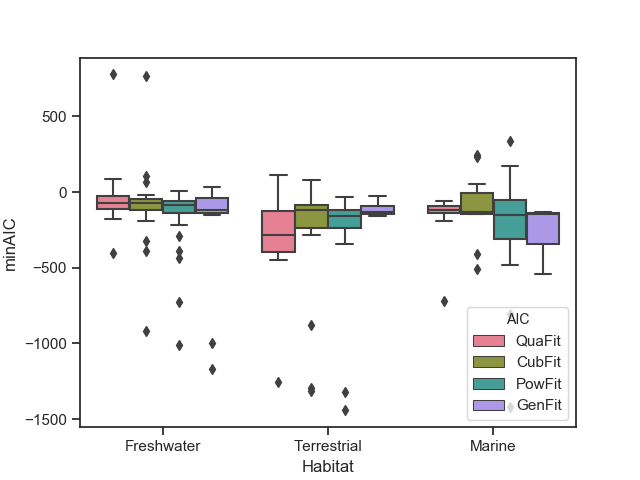
\includegraphics[]{HabitatCompare.png}
	\caption{Habitat Clustered Boxplot}
	\label{Habitat Clustered Boxplot}
	
\end{figure}


\begin{figure}[h!]
	
	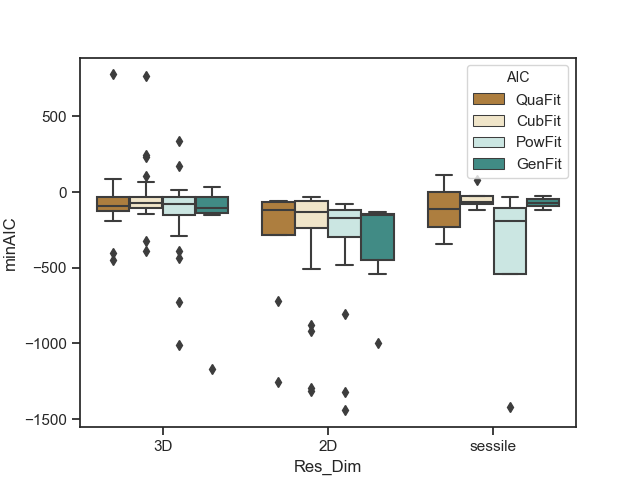
\includegraphics[]{Res_Dim_Compare.png}
	\caption{Resource Dimensionality Boxplot}
	\label{Resource Dimensionality Boxplot}
	
\end{figure}

Comparing the different habitat model fits showed minimal variation in the ideal model fit 


	\section{Discussion}
\noindent

How well do different mechanistic and phenpmenological mathmathical models fit functional response data across different species?
Overall, the mechanistic models fit 20\% more functional responses than phenmeonological. However, 


Another aspect of the study which was overlooked was the taxa that the species were placed, the phylogeny of a species has been shown to impact types of functional responses, a study by Robert P.Dunn in 2020 discussed the importance of including taxa, especially of the predator, when looking at model fits of functional responses

	
\newpage


\vspace*{1\baselineskip}
\printbibliography 


\newpage

\end{document}